\documentclass{sig-alternate}


\usepackage{algorithm}
\usepackage{algorithmic}
\usepackage{amsmath}
\usepackage{amssymb}
\usepackage{array}
\usepackage{booktabs} 
\usepackage{cases}
\usepackage{enumitem}
\usepackage{epstopdf}
\usepackage{graphicx}
\usepackage{listings}
\lstset{
  basicstyle=\ttfamily,
  columns=fullflexible,
  frame=single,
  breaklines=true,
  postbreak=\mbox{\textcolor{red}{$\hookrightarrow$}\space},
}
\usepackage{longtable}
\usepackage{makecell}
\usepackage{multirow}
\usepackage{stfloats}
\usepackage{subeqnarray}
\usepackage{xcolor}
\usepackage{diagbox}

\lstset{
    escapeinside={(*}{*)}
}

%\usepackage{authblk}
\usepackage[caption=false,font=footnotesize]{subfig}

\newtheorem{problem}{Problem}

%\setcopyright{rightsretained}

% DOI
%\acmDOI{10.475/123_4}

% ISBN
%\acmISBN{123-4567-24-567/08/06}

%Conference
%\acmConference[MobiCom'18]{}{}{}
%\acmYear{2018}
%\copyrightyear{2018}

%\acmPrice{15.00}

%
\def\sharedaffiliation{%
\end{tabular}
\begin{tabular}{c}}
%

\newcommand{\sdn}{Malak}


\newcommand{\simpleTput}{80\%}    % overall throughput
\newcommand{\simpleLife}{20\%}    % lifetime increase using basic routing
\newcommand{\diagLife}{25\%}      % lifetime increase using diagnosis
\newcommand{\seleLife}{35\%}      % lifetime increase using selection algo.
\newcommand{\totalLife}{80\%}     % total increase using both diagno and selec algo
\newcommand{\pktRecvRatio}{80\%}  % packet recieved ratio


\begin{document}

\title{{\sdn}: An Intelligent, High-performance and Resilient Software Defined Wireless Sensor Network System}
\author{}

%energy exhaustion


\maketitle

\begin{abstract}

Software defined network (SDN) enables  
artificial intelligence (AI) techniques to be implemented easily, and in
turn AI techniques greatly improve the performance and resilience of SDN system.
However, all the existing SDN systems in wireless sensor networks are implemented
in simulators and there is no practical implementation.

In this paper, we present {\sdn}, the first practical SDN wireless sensor network system,
which achieves intelligence, high-performance and resilience simultaneously.
In {\sdn}, we utilize a set of unmanned aerial vehicles (UAVs) to serve as the SDN controllers. 
UAVs communicate with sensor nodes by one-hop communication and thus greatly
reduce the network energy consumption. 
We designed easy-to-use interfaces and implemented five SDN applications, namely
routing, multi-task, network diagnosis, AI energy exhaustion prediction, AI node selection.
{\sdn} is a ecosystem that all applications can run simultaneously to benefit each other.
Our evaluations show the throughput improves by {\simpleTput} compared with two notable protocols.
%by using the basic {\sdn} routing algorithm. 
Meanwhile, the average lifetime of sensor nodes grows by
{\simpleLife}. By running energy prediction %and AI selection 
application, {\sdn} further increases the lifetime by {\totalLife}. %and {\seleLife}
All source code and results of {\sdn} are ready to open source.



%throughput improves by 1.2X compared to two notable traditional sensor network routing protocols.

%throughput    comparing with other provence,  still maintains initial throughput 
%when  


%!TEX encoding = UTF-8 Unicodestate-of-the-art

\end{abstract}
  
\section{Introduction}

Why we are SDN ?

Software defined network is able to support flexible network programmability 
by using programmable data plane and centralized network controller.

OpenFlow focus on wired networks.

Challenges and opportunities of SDN for WSN:

Challenges: Limited resources of WSN nodes:
\begin{itemize}
\item	energy
\item	processing
\item	memory
\item	communication
\end{itemize}

Opportunities: 
\begin{itemize}
\item	Improve resource reuse
\item	Implement node retasking 
\item	Node and network management
\item	Enable experiments with new protocols
\end{itemize}



Why and How we can implement AI ?

How we combine Ai with other applications?


AI 

AI systems have been improving, and new advances in machine intelligence are creating seamless interactions between people and digital sensor systems.

 In sensor systems, applications can be found for a variety of tasks, including selection of sensor inputs, interpreting signals, condition monitoring, fault diagnosis, machine and process control, machine design, process planning, production scheduling, and system configuring. Some examples of specific tasks undertaken by expert systems are:
* Assembly 
* Automatic programming 
* Controlling intelligent complex vehicles  
* Planning inspection 
* Predicting risk of disease 
* Selecting tools and machining strategies 
* Sequence planning 
* Controlling plant growth. 

.



The tools and methods described have minimal computation complexity and can be implemented on small assembly lines, single robots, or systems with low-capability microcontrollers. These novel approaches proposed use ambient intelligence and the mixing of different AI tools in an effort to use the best of each technology. The concepts are generically applicable across many processes.


minimum energy, data loss, reliability, robustness, etc., in place during the design and operation of wireless sensor networks

a specific set of protocols for medium access, localization and positioning, time synchronization, topology control, security and routing are identified based on the current configuration of the network, the requirements of the application and the topology of their deployment.
\section{Related work}

\subsection{Software Defined Wireless Sensor Networks}


There are several existing SDN approaches for sensor system, 
namely flow sensor \cite{mahmud2011exploitation}, SDWN \cite{costanzo2012software},
sensor openflow \cite{luo2012sensor}, TinySDN \cite{de2015tinysdn}, SDN-WISE \cite{galluccio2015sdn}.
However, they are all implemented and evaluated only in simulators. 

\textbf{Flow Sensor.}
The previous idea presented in paper \cite{mahmud2011exploitation} addresses 
reliability in the sensor networks through exploiting the OpenFlow technology\cite{Mckeown2008OpenFlow}. 
Coming up with the concept of flow-sensor instead of typical sensor \cite{Liu2015Thermoresistive}, 
they have successfully made it possible to achieve communications between controller, 
gateway and sensors. Besides, they proved flow sensor to be more 
reliable since data packets, control packets and the sensor nodes 
themselves can be easily monitored, regulated and routed whenever 
required. Therefore, a robust routing and uninterruptible messages 
flow of sensors are achieved. The results described in this paper 
shows flow-sensor is able to display much better performance even for large networks.

\textbf{SDWN.}
The solution of supporting the SDN approach in LR-WPANS is first presented in \cite{costanzo2012software}. 
Given the gap that advantages of SDN and the proper ways to expand it to wireless networks are not clear enough, 
the group analyzes the opportunities of SDN-related wireless network and illustrates 
the requirements should be considered to utilize SDN solution for wireless networks. 
They made a good attempt to develop the SDWN protocol stack.

\textbf{Sensor OpenFlow.}
In the paper \cite{luo2012sensor}, the group took a radical, yet backward 
and peer compatible approach to tackle the problems existing in WSN 
such as resource underutilization, counterproductive, rigidity to policy 
change and manage difficulty. They propose SD-WSN with a separation between 
data plane performing flow-based packet forwarding and control plane performing network control. 
The core part designed is Sensor OpenFlow(SOF), which gives a standard protocol for the communication 
between data and control part. Based on the whole architecture they gave, 
the underlying network becomes programmable by using SOF.

\textbf{Tiny SDN.}
TinySDN \cite{de2015tinysdn} is a TinyOS-based SDN framework aiming to 
address the problem that only single controller can be coupled to the sink. 
Besides, TinySDN is a hardware independent framework that comprises two parts: 
SDN-enabled sensor node and SDN-controller node. 
In order to test the reliability of this framework, the authors conducted some experiments on COOJA. 
Through analyzing results concerning delay and memory 
footprint, they found it is feasible in communication provided by SDN paradigm.

\textbf{SDN-WISE.}
One solution for wireless sensor network is introduced in the paper \cite{galluccio2015sdn}, 
and the authors implement the prototype of this idea. Compared to other SDN solutions for wireless network, 
this solution successfully reduces the message exchange needed between sensor nodes and controller. 
Besides, flexible APIs are provided by the authors, which makes the network much easier to program. 
Also, they implemented some experimental testbed, and found that in a power limited hardware, the response delay was still very small. 
SDN-WISE shows its good performance in different operation conditions. However, SDN-WISE only validates its performance in simulators. 


\subsection{Applications for Wireless Sensor Networks}


There are already a rich set of the applications for WSNs. 
However, we study the typical applications and find that
distributed fashions for WSN cannot 
promise global optimization. %without the support of SDN.
Worse, no existing work can combine different applications to run together.
To design a ecosystem for software defined sensor networks, we are to implement applications of
routing, network diagnosis, AI sensor, sensor selection and multi-task.




\textbf{Routing.}
Low-power and lossy network consists of devices whose processing capability, 
memory and energy are constrained \cite{Winter2012}. Hence, traditional 
protocols cannot be used there. However, RPL is one of the standards for IPv6\cite{Deering1998Internet} routing in LLN. 
It builds the topology in form of a tree, performing DAO, DIO, ACK to generate a directed acyclic graph 
from one or more roots to the leaf nodes. The experiments done in the paper \cite{Tsiftes2010a} show 
that IPv6 routing with ContikiRPL is both lightweight and power-efficient.
 
\textbf{Network Diagnosis.}
Previous diagnosis algorithms share the same drawback 
that their process of gathering information is static and the reports sent to be 
analysis are not intermediate enough \cite{Ramanathan2005Sympathy,Khan2010Diagnostic}. 
Directional Diagnosis \cite{gong2015directional} is an online diagnosis approach to dynamically 
recognize the most useful information according to an engine designed in the approach. 
Besides, the diagnosis process only focuses on the problematic area, 
thus it can produce a more accuracy prediction \cite{Pavlou2015How}. 
Specifically, the whole approach consists of four main parts: 
node tracing, trace collection, inference model and incremental probing. 
The node tracing algorithms dynamically reconstruct the topical topology and derive inner dependencies. 
Based on the collected data information, inference model can guide the next probe 
by incremental probing upon belief network. The experiments done show the diagnosis 
process promises high efficiency in real time.

\textbf{AI sensor.}
The application of sensors often relays on the fields 
like sensor selection and data prediction with the help of AI algorithms. 
In order to select the subset of nodes to be active, related study gives a way to dynamically 
response to the change of sensor network based on the historical information \cite{Mo2013Dynamic}.
The new sensor node has a different time factor from the old 
node when constructing the predictive network. 
Besides, the position of nodes may be sufficiently used to reduce the weight of 
nearby nodes in a predictive network \cite{Kumar2017Edge}. 
As for the data prediction, on the one hand, the energy consumption information 
can be collected. Previous work on diagnosis, for example, only performs 
diagnosis process when sensors almost run out of energy. On the other hand, the original 
data on temperature, humidity, light intensity is a reliable resources for 
prediction in time series\cite{Raza2014Practical}. 

\textbf{Sensor Selection.}
Redundant sensor network always contains nodes that generating data 
stream with some overlapping parts \cite{Ali1995Redundant}. 
Collected information can be useful to determine which sensors are active. 
The algorithms come up with in paper\cite{li2016spatially} are called Spatially Regularized Streaming Sensor Selection(SRSSS). 
The authors not only consider the spatial information but also the historical obversion of the sensor network. 
They apply higher weights to nearby sensors and introduce a time-forgetting factor \cite{Astrom1989Adaptive} so that their approach can predict more accurately and response much faster.
	
\textbf{Multi-task.}
One single sensor node may shoulder several tasks. To save the energy consumption of the network, 
when a task is assigned, we need to choose which sensor to be active and which to be inactive \cite{Georges2011Energy}. 
Nowadays, works aiming to design an energy-efficient sensor management strategy
tends to develop their methods in three steps: choose the proper subset of nodes to be active \cite{Aghdasi2009High}, choose the subset of active nodes to assign the task and set the sampling rate of the task. Related study has found an efficient online 
algorithm considering sensor activation and task mapping to deal with dynamic events during the 
runtime of software defined sensor network system \cite{Zeng2015}.

\section{Architecture}
\label{Arc}
Before introduce our SDN system architecture, we first lead into some basic terms in SDN system,.

\textbf{Data plane}: forwarding data and basic sensing functions.

\textbf{Control plane}: the protocols used to populate the forwarding tables of data plane elements.

\textbf{Management plane}: software services. network policy is defined in management plane, the control plane enforces the policy, and  the data plane executes it by forwarding data accordingly. (running applications)

\textbf{Southbound Interface (SI)}: The instruction set of the forwarding devices is defined by the southbound API, which is part of the southbound interface. Furthermore, the SI also defines the communication protocol between data plane and control plane elements. This protocol formalizes the way the control and data plane elements interact.

\textbf{Northbound Interface (NI)}: The middleware on control plane can offer an API to application developers. This API represents a northbound interface, i.e., a common interface for developing applications. Typically, a northbound interface abstracts the low-level instruction sets used by southbound interfaces to program forwarding devices.

The architecture of {\sdn} is shown in Fig. \ref{Architecture}. 
The system is divided into three layers: data plane, 
control plane and management plane respectively.

\begin{figure}[htbp]
	\centering
	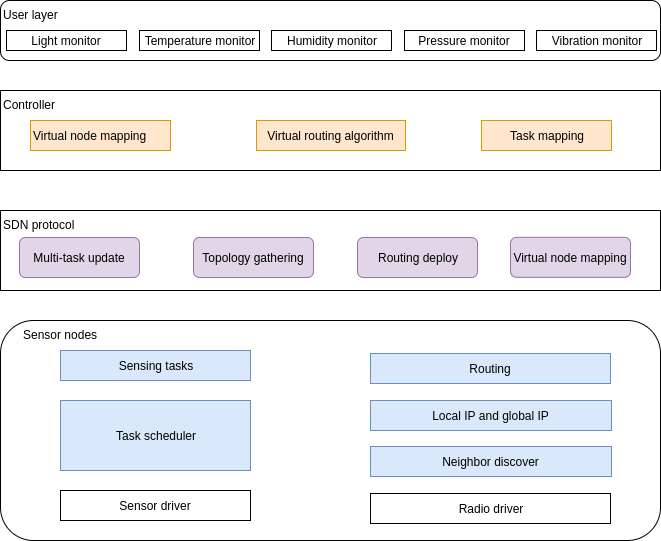
\includegraphics[width=3.5in]{./Figure/Architecture}
	\caption{Architecture of the system.}
	\label{Architecture}
\end{figure}

To build software defined network system in WSN and achieve low 
energy consumption and high performance, the SDN controller ought to  
configure data plane within as less hops as possible.  
In {\sdn}, we choose UAV as a mobile SDN controller,  
which communicates with sensor nodes by on-hop communication.
It significantly reduces the energy consumption of nodes in {\sdn}. 
To achieve high performance, the UAV controller carries
a powerful airborne computer which has ability to run 
some intelligent applications in real-time.

The \textbf{data plane} runs on sensor nodes while the control 
plane and management plane run on UAV controller. 
And the interface between data plane and control plane is defined as southbound interface,
while the interface between control plane and management plane is defined as southbound interface.

In the \textbf{control plane}, in order to make our system easy to use,  we implement a database on the UAV and design interfaces for data plane and SDN applications. The control plane connected data plane and 
management plane. The database maintain the topology gathered from the data plane, route table inputed form applications, and sensor task schedule table form management application.

On \textbf{management plane}, user can run tons of applications base on our well-defined southbound APIs, such as routing algorithms, network diagnose, sensor task 
scheduler, etc.


Different from wired network, the data plane of WSN not only runs
data forwarding function, but also executes data sampling function. 
For example,  sensor nodes execute neighbor discovery process for getting topology, 
data sampling process for getting data from environment and data forwarding process
for data gathering. In {\sdn} is a easy-to-use system that we design and implement a lot of 
interfaces for users.

As shown in Fig \ref{downstream} and Fig \ref{upstream}, the southbound data structure fully considered the difference between wired networks and wireless sensor networks, the data structure not only contains routing  related data, but also has sensor task control tables.

\begin{figure}[htbp]
	\centering
	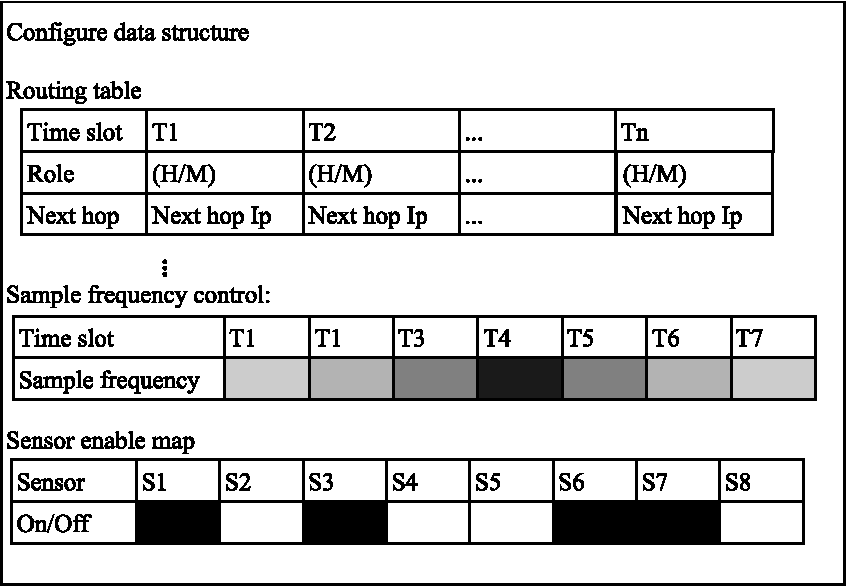
\includegraphics[width=1\columnwidth]{Figure/downstream}
	\caption{Downstream data structure}
	\label{downstream}
\end{figure}

\begin{figure}[htbp]
	\centering
	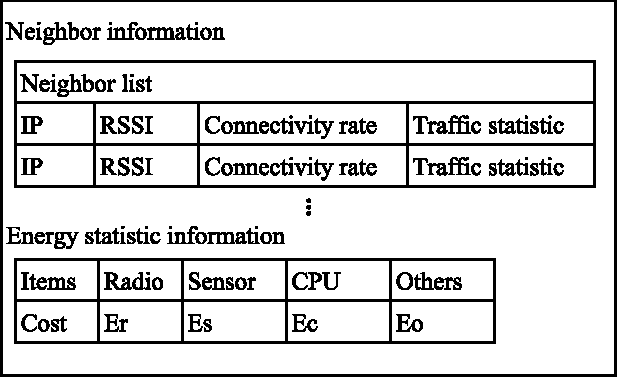
\includegraphics[width=1\columnwidth]{Figure/upstream}
	\caption{Upstream data structure}
	\label{upstream}
\end{figure}



The Table \ref{API} shows our southbound interface for user write applications. By using our SDN Southbound Interface, user can easy to write 
a variety of applications, such as routing protocol, sensor task scheduler, network diagnose, algorithm evaluator, etc.
\begin{table*}[!b]
	\caption{SDN Southbound Interface}
	\label{API}
	\centering
	\scalebox{0.9}{
	\begin{tabular}{|l|l|}
		\hline
		\makecell[tc]{\textbf{Structure \&\& Function}} & \makecell[tc]{\textbf{Description}} \\
		\hline
		\multicolumn{2}{|c|}{\textbf{Sensor Control Interface}}\\
		\hline
		\hline
		struct node & Sensor node structure\\
		\hline
		struct nodeset & A set of sensor nodes \\
		\hline
		struct neighbor\_list & Neighbor infomation \\
		\hline
		struct energy\_item & Energy statistic information \\
		\hline
		struct rout\_table & Route table \\
		\hline
		struct duty\_cycle\_table & Duty cycle control table \\
		\hline
		struct sensor\_enable\_table & All the nodes's states. Node state: \{on,off\} \\
		\hline
		switch\_node(node,state) & Turn on or turn off the node \\
		\hline
		get\_node\_info(node) & Get node's information, including  node's position, duty cycle, power, etc.\\
		\hline
		set\_node\_attr(node,attrTag,value) & Set node attribute, including  duty cycle, radio strength, etc. \\
		\hline
		get\_neighborlist(node) & Get the neighbor list of a node \\
		\hline
		\multicolumn{2}{|c|}{\textbf{UAV Application Interface}}\\
		\hline
		\multicolumn{2}{|c|}{\textbf{Routing}}\\
		\hline
		\hline
		get\_topology() & Get the topology of the network\\
		\hline
		get\_rout\_table(node) & Get the route table of a node \\
		\hline
		set\_route(node) & Set the route of a node \\
		\hline
		\multicolumn{2}{|c|}{\textbf{AI Node selection}}\\
		\hline
		\hline
		nodeset simple\_selection(nodeset) & Select sensor set by location information\\
		\hline
		nodeset SRSSS\_selection(dataset) & Select sensor set by AI algorithm based on sensing data\\
		\hline
		\multicolumn{2}{|c|}{\textbf{AI Energy Prediction}}\\
		\hline
		\hline
		model\_selsct(modeltype) & Select an AI model\\
		\hline
		model.train(dataset,ratio) & Train an AI model with learning ratio on the data set\\
		\hline
		model.test(dataset) & Test the AI model on the data set\\
		\hline
		model.predict(node) & Do the energy prediction for a node \\
		\hline
		\multicolumn{2}{|c|}{\textbf{Multi-tasks}}\\
		\hline
		\hline
		create\_scheduler() & Create a task scheduler \\
		\hline
		scheduler.create\_buffer() & Create a task buffer \\
		\hline
		scheduler.task\_buffer\_add(task,nodeset) & Add a new task to task buffer \\
		\hline
		scheduler.task\_buffer\_remove(task) & Remove a new task to task buffer \\
		\hline
		scheduler.task\_buffer\_update(task,nodeset) & Update a task to task buffer with a new nodeset \\
		\hline
		scheduler.task\_update() & Schedule the added or removed tasks in the buffer\\
		\hline
		\multicolumn{2}{|c|}{\textbf{Diagnosis}}\\
		\hline
		\hline
		detect() & Detect problematic region with probes \\
		\hline
		get\_topical\_topology(nodeset) & Construct topical topology\\
		\hline
		diagnose\_network(topology,nodeset) & Diagnose the failure nodes or lossy links\\
		\hline
	\end{tabular}
	}
\end{table*}

We demonstrate two application code using our southbound interface. The List. \ref{topology-update} shows a deployed routing algorithm based on our SI. 
And the List. \ref{AI} demonstrate a AI selection and Muti-tasks application.

\begin{lstlisting}[
	language={[ANSI]C},
	label=topology-update,caption={An example of deploy routing algorithm},
	keywordstyle=\color{blue!70},
	showstringspaces=false,
	commentstyle=\color{red!50!green!80!blue!70},
	frame=single,captionpos=t,
	rulesepcolor=\color{red!20!green!20!blue!20},
	basicstyle=\ttfamily]
topology = get_topology();
//calculate route table for each node
//based on topology
for(node=0; node<nude_num; node++){
   node.routingtable =
      calculate_routable(topology);
}
//set route table for each node
for(node=0; node<nude_num; node++){
   fly_to(node);
        set_route(node.routingtable);
}

\end{lstlisting}

\begin{lstlisting}[language={[ANSI]C},label=AI,
	caption={An example of AI selection and Muti-tasks},
	keywordstyle=\color{blue!70},
	showstringspaces=false,
	commentstyle=\color{red!50!green!80!blue!70},
	frame=single,captionpos=t,
	rulesepcolor=\color{red!20!green!20!blue!20},
	basicstyle=\ttfamily]
AI_Multitasks(taskset){
   create_scheduler();
   scheduler.create_buffer();

   for(task=taskset.head; task < taskset.len;task=task.next)
      scheduler.task_buffer_add(
         task,
         defaultset);

   scheduler.task_update();
   ...
   ...
   while((task = scheduler.task_next)!= NULL){
      data = get_collected_data();
      nodeset =
         SRSSS_selection(dataset);
      scheduler.task_buffer_update(
         task,
         nodeset);
   }
   scheduler.task_update();
}

\end{lstlisting}


%\section{Network construction}

\subsection{Sensor selection}
ssss
Physical topology :  uniform distribution (Density ρ).

Sensor selection algorithm:
\begin{itemize}
\item[1)] A simple cluster algorithm: threshold δ -The distance between sensors \&\& the overlapping of sensing area \&\& the similar neighbor list. 
\item[2)] SRSSS Algorithm (AAAI-16) - trained by an AI model based on the collected data. 
\end{itemize}

Output : Redundant nodes

\subsection{Topology Mapping}

Redundant nodes are mapped to a virtual node. 
They can awaken each other according to their  residual energy. 
When:    
$$
\begin{aligned}                        
ResidualEnergy(i) \leq \xi \cdot ResidualEnergy(j) & &   {turn~node~i~to~node~j}\\
\end{aligned}
$$

These virtual nodes are called critical nodes in the logical topology while other nodes are called ordinary nodes.

\subsection{Logical routing}

Critical nodes first (CNF) algorithm
\section{Applications}

\subsection{Overview}

Traditional applications can not achieve complicated and efficient goals due 
to the limited processing power and memory space of sensors.

In {\sdn}, applications for wireless sensor networks are inspired by 
greater potential with the UAV based SDN controller. The central controller
helps sensors execute complex calculations such as AI model training, as well 
as store global information. Besides, UAVs have flexible features and can deploy 
tasks to sensors by one-hop communication directly. Thus it enables the sensor network
to achieve much more intelligent applications.

In {\sdn}, applications can be found for a variety of purposes, including routing, AI node selection,
AI energy prediction, multi-tasks and network diagnosis. We design all these applications and provide 
easy-to-use interfaces to users as in Table \ref{API}.


\newpage
\subsection{Routing}

one round

cluster header

\begin{table}[htbp]
	\caption{Flow Table}
	\label{FT}
	\centering
	\scalebox{0.9}{
	\begin{tabular}{|l|l|l|}
		\hline
		Header Fields & Counters & Actions \\
		\hline
		\end{tabular}
	}
\end{table}

\begin{table}[htbp]
	\caption{Header Fields}
	\label{HF}
	\centering
	\scalebox{0.9}{
	\begin{tabular}{|l|l|l|l|l|}
		\hline
		Ingress port & Ether Source & Ether Dst &IP src & IP dst \\
		\hline
		\end{tabular}
	}
\end{table}

Actions:
\begin{itemize}
\item	Forward
\item	Drop
\item	Report
\item	Forward
\item	Drop
\item	Report
\item	Drop
\item	Report
\end{itemize}

\newpage
\subsection{Network Diagnosis}

\subsubsection{Motivation}

Sensor nodes are provisioned with low-capacity batteries and will run out of energy in the end. 
Besides, uncertain environmental factors will lead to the failure of communications.
Upon these two factors, there occurs network faults such as failure nodes and lossy links from time to time.

Network fault diagnosis is then designed to help network administrators monitor the network 
operational status and maintain a sensor network system. The key idea of the existing works
on fault diagnosis is to collect running information from nodes and deduce root causes of network
exceptions. The running information is collected by a mechanism of probing.

We implement the network diagnosis process as an application in our {\sdn} system.
Since in {\sdn} we have our mobile UAV as a controller, a more flexible way is to infer the suspicious 
nodes of the network fault in traditional way first and then set the UAV to check out the fault sources. 
 
\subsubsection{Design}

We first introduce a state-of-the-art algorithm named DID 
\cite{gong2015directional}, which is a directional diagnosis approach.
We utilize the node tracing module and the tracing collection module of DID
to infer the suspicious nodes in our network diagnosis application, 
and then set our UAV controller to confirm the network elements being faulty.

The node tracing module is conducted in each sensor node. 
Every time a packet arrives at a node, it counts
the source of the packet . The tracing collection module
is set in the UAV controller. When network exception is detected, 
it gathers the tracing information in the tracing module of the relevant nodes
and infers a suspicious node set. Next we set the UAV to fly through the 
node set and check each node first to diagnose the failed nodes. 
Then UAV collects the neighbor lists of all the nodes in the suspicious node set.
With the collected neighbor lists, the UAV controller reconstructs the topical topology and 
compares it with the default topology to find the failed links.

Compared to DID, the diagnosis application in {\sdn} releases the complicated inference
computations and can achieve accurate diagnosis since the UAV can fly to the sensors 
to confirm the network faults. {\sdn} can realize the four types of fault sources the same as DID:  
\begin{itemize}
\item	Node failure. This network failure is caused by the node itself.
\item	Link failure. This network failure is caused by the communication links 
between nodes, mainly relating to traffic flow in networks.
\item	Temporary failure. This  network failure is caused by complex interior or exterior 
interferences and quick self-recovery
\item	Multiple failures. This  network failure is caused by multiple failures above.
\end{itemize}



\subsection{AI Node Selection}

\subsubsection{Motivation}

It is inevitable that there will be a part of redundant sensors when deploying a 
practical wireless sensor network. These redundant nodes have overlaps of
observation regions, and what makes the matter worse is that redundant nodes
may cause great communication interference. Therefore it is significant to select 
proper sensors to avoid data redundancy and save the sensor network energy consumption.

In {\sdn}, we provide the node selection application to users. The SDN controller executes the 
selecting algorithm and send the control instructions to activate the selected nodes.

\subsubsection{Design} Our {\sdn} system provide two main node selecting methods: 
greedy selection algorithm and SRSSS algorithm. This application will be extended to more elegant 
algorithms in our future work. 

\textbf{Greedy selection algorithm.} We first provide a simple method to select 
the redundant nodes by a greedy selection algorithm, as described in Alg. \ref{Greedy}. 
The key idea is to select nodes as less as possible to coverage the whole area
 based on the location and sensing range. 
 
 We implement the greedy selection algorithm in {\sdn}. The evaluations in section \ref{Eva} 
 show it greatly saves the sensors' energy and thus prolongs the network lifetime.

\begin{algorithm}
\caption{Greedy Selection Algorithm}
\label{Greedy}
\begin{algorithmic}[1]
\STATE Input: Sensor set $N$, Selected set $M$, Target area $\Omega$, Covering area $\Phi$;
\STATE Initialize : $M = \emptyset$, $\Phi = \emptyset$
\WHILE {$M \neq N$}
    \IF{$\Phi = \Omega $}
        \STATE break; $\backslash$$\backslash$ Selected set has been found
    \ENDIF
    \IF{$\forall n_i \in (N-M) : range(n_i) \subset \Phi$}
    	 \STATE break;$\backslash$$\backslash$ Cannot cover the target area;
    \ENDIF
    \STATE Find $n_i : argmax(\Phi \cap range(n))$, $n_i \in (N-M)$;
    \STATE $\Phi = \Phi \cup {n_i}$
\ENDWHILE
\STATE Output: $M$;
\end{algorithmic}
\end{algorithm}

\textbf{Spatially regularized streaming sensor selection (SRSSS).} 
To realize more intelligent and effective sensor selection, we introduce 
a state-of-the-art AI algorithm named spatially regularized streaming 
sensor selection (SRSSS) proposed in \cite{li2016spatially}.

Different from the greedy selection algorithm, SRSSS is a multi-variate 
interpolation framework and focuses on selecting a subset
of sensors in a streaming scenario to minimize collected information redundancy.  

Traditional wireless sensor network is not suitable to implement an AI selection approach
due to the limited computational capability of sensors. Some work use the database to collect data
and make decisions by multi-hop communications. However, in this way the network will use up a great deal of energy.
In our {\sdn}, the UAV fly through the nodes to pick up the collected data and executes the computations.
Then it sends the control instructions to the nodes by one-hop communication and greatly saves the network energy.

The aim of SRSSS is to optimize its objective function which is an equation given
certain constraints of collected information, location and energy consumption.
The objective function is formulated as:

\begin{equation}
\label{OF}
\begin{aligned}
& (W_{k+1},z_{k+1})  \\
& = arg \min_{W,z} \sum_{i=1}^k \mu^{k-i}\lVert X_k^iD_zW(I-D_z)-X_k^i(I-D_z)\rVert^2_2 \\
& + \alpha\sum_{i,j=1}^n\lVert y_i-y_j\rVert_2\lvert W_{i,j} \rvert - \beta\sum_{i,j=1}^n\lVert y_i-y_j\rVert_2 z_iz_j \\
& + \lambda\lVert W \rVert^2_F \\
&s.t. z = [z_1,...,z_n] \in {\{0,1\}}^n, c^Tz \leq P
\end{aligned}
\end{equation}

The first term in (\ref{OF}) is to minimize the prediction error of the collected data
and the following two terms incorporate spatial information. The last term constrains
the complexity of the learned matrix $W$. The energy constraint is controlled by 
the inequality in (\ref{OF}). Because of the limitation of length,  we leave out all the details. 
The meaning of the parameters and the mechanism of 
SRSSS can be seen in \cite{li2016spatially}. 

With the AI sensor selection process, {\sdn} becomes a smarter and adaptive sensor systems. 


\iffalse
\newpage
\subsection{AI Energy Prediction}

\subsubsection{Motivation}

\subsubsection{Design}
\fi

\newpage
\subsection{Multi-tasks}

\subsubsection{Motivation}

Wireless sensor networks (WSN)  generally comprise of a group of 
spatially dispersed sensors. In a wireless sensor network, 
sensor nodes are equipped with various 
types of sensors monitoring and recording 
environmental conditions like temperature, sound, sunlight,
humidity, etc.

A given sensing task involves multiple sensors to 
achieve a certain quality-of-sensing.
Generally, an efficient task scheduling for the nodes is that nodes 
are able to perform multiple tasks simultaneously. 
For example, sensors deployed in a grove are assigned tasks to collect
sunlight, temperature and humidity data and these tasks require different 
number of  nodes with respective sensing range, rate and duration.
However, traditional sensor networks are not suitable to conduct this 
multi-tasks due to the limitations of computation complexity for task 
arrangement of each node.

In our {\sdn} system, we implement the multi-tasks application 
with the help of the central controller. The SDN controller
maintains programmable task scheduling and management
modules while sensor nodes are loaded with interfaces to
receive task control instructions.     

\subsubsection{Design}

A deployed wireless sensor networks are usually assigned  with
different data collection requirement. In {\sdn}, we design and 
implement multi-task application and provide easy-to-use
interfaces to users.

When a user assign a task to {\sdn}, the UAV controller will first check out 
the energy and storage constraints of the required sensor set, as described in Alg. \ref{}. 
If the task requirement exceeds the capacity of the sensor set, it will be sent to a     
task queue; Otherwise it will be put into the task buffer to conduct.


\begin{algorithm}
\caption{Sensor Constraint Detection}
\label{Constraint}
\begin{algorithmic}[1]
\STATE Input: Sensor set $N$, Selected set $M$, Target area $\Omega$, Covering area $\Phi$;
\STATE Initialize : $M = \emptyset$, $\Phi = \emptyset$
\WHILE {$M \neq N$}
    \IF{$\Phi = \Omega $}
        \STATE break; $\backslash$$\backslash$ Selected set has been found
    \ENDIF
    \IF{$\forall n_i \in (N-M) : range(n_i) \subset \Phi$}
    	 \STATE break;$\backslash$$\backslash$ Cannot cover the target area;
    \ENDIF
    \STATE Find $n_i : argmax(\Phi \cap range(n))$, $n_i \in (N-M)$;
    \STATE $\Phi = \Phi \cup {n_i}$
\ENDWHILE
\STATE Output: $M$;
\end{algorithmic}
\end{algorithm}


A sensor node may have different sensing ranges for different tasks.


There are several practical requirements.

Different tasks have different requirements, including time, sensing range, sensing ratio, etc.

For example tasks like sunlight collection only need to be carried out during the daytime.

Our system provide a task scheduling to 

Sensors are usually assigned multi-tasks.

Sensors are assigned tasks to monitor a specific area.

\begin{table*}[htbp]
	\caption{Task Buffer}
	\label{TB}
	\centering
	\scalebox{0.9}{
	\begin{tabular}{|l|l|l|l|l|}
		\hline
		Task ID& Node set& Sensing rate & Sensing range& Sensing duration \\
		\hline
		Task ID& Node set& Sensing rate & Sensing range& Sensing duration \\
		\hline
		...& ...& ... & ...& ... \\
		\hline
		Task ID& Node set& Sensing rate & Sensing range& Sensing duration \\
		\hline
		...& ...& ... & ...& ... \\
		\hline
		\end{tabular}
	}
\end{table*}

Different tasks have different requirements, i.e. 

\begin{itemize}
\item \textbf{Node set.} Users can assign tasks to 
\item \textbf{Sensing rate.}
\item \textbf{Sensing range.} The maximum distance that a node can detect. 

\item \textbf{Sensing duration.} The sensing time from start to end. 
There is no need to collect sunlight data at night.
\end{itemize}

Task scheduler do the arrangement. 

Task buffer.

Task queue.

Scheduling table.

...


\section{Implementation}
\label{Imp}



\subsection{Data Plane}

We run modified contiki-ng, a system for next generation IoT (Internet of
Things), on data plane. We modify the network layer of contiki-ng, and abstract
data plane interface to separate network control functions from data plane. 
The details are described as follows.

\textbf{Neighbor Discovery}: After deployment, nodes frist start IPv6 neighbor
discovery protocol to find the nodes which can be reached within one hop, and
then save the neighbor information to neighbor table and wait for UAV arriving
to gather the topology information. Every neighbor's information consists of the
neighbor's IP and RSSI. 

\textbf{Packet Forwarding and Data Sampling}: The nodes get routing table from UAV through
northbound interface. When a node receive a data packet from other nodes, it
just sends it to the next hop node according the roSuting table.

Nodes read task table received from UAV to decide when
to wake up sensors to make sure that they cost minimal energy to get the same
quality data. 

\subsection{Control Plane}

We run our SDN control plane a power airborne computer carried by UAV. 
The UAV's flight controller runs on ROS (Robot Operating System) base on UAV's SDK.
And we use MySQL as our SDN database. UAV gathers topology from each node and save
it into database, so that users can easily read the whole network data from
database. For the same reason, after a user gets routing algorithm results and
saves it into database via northbound interface, our control plane will
automatically divides the whole network routing results into individual node's
routing table, and then sends it to specific nodes.

\subsection{Hardware Platform}

Based on our software framework, we use DJI M100 UAV carrying Nvidia TX-2 airborne
computer, and adapt 250 TI CC2650 SensorTag to build our testbed. The TX-2 built around an NVIDIA GPU 
and loaded with 8 GB of memory and 59.7 GB/s of memory bandwidth. It is most power-efficient embedded 
AI computing device which is suitable for UAV onboard computing. The SensorTag communicate with UAV and
other nodes through Zigbee stack, it also equip with 10 different kid of sensors which is suitable for 
large scale wireless sensor networks.

\begin{figure}[htbp]
	\centering
	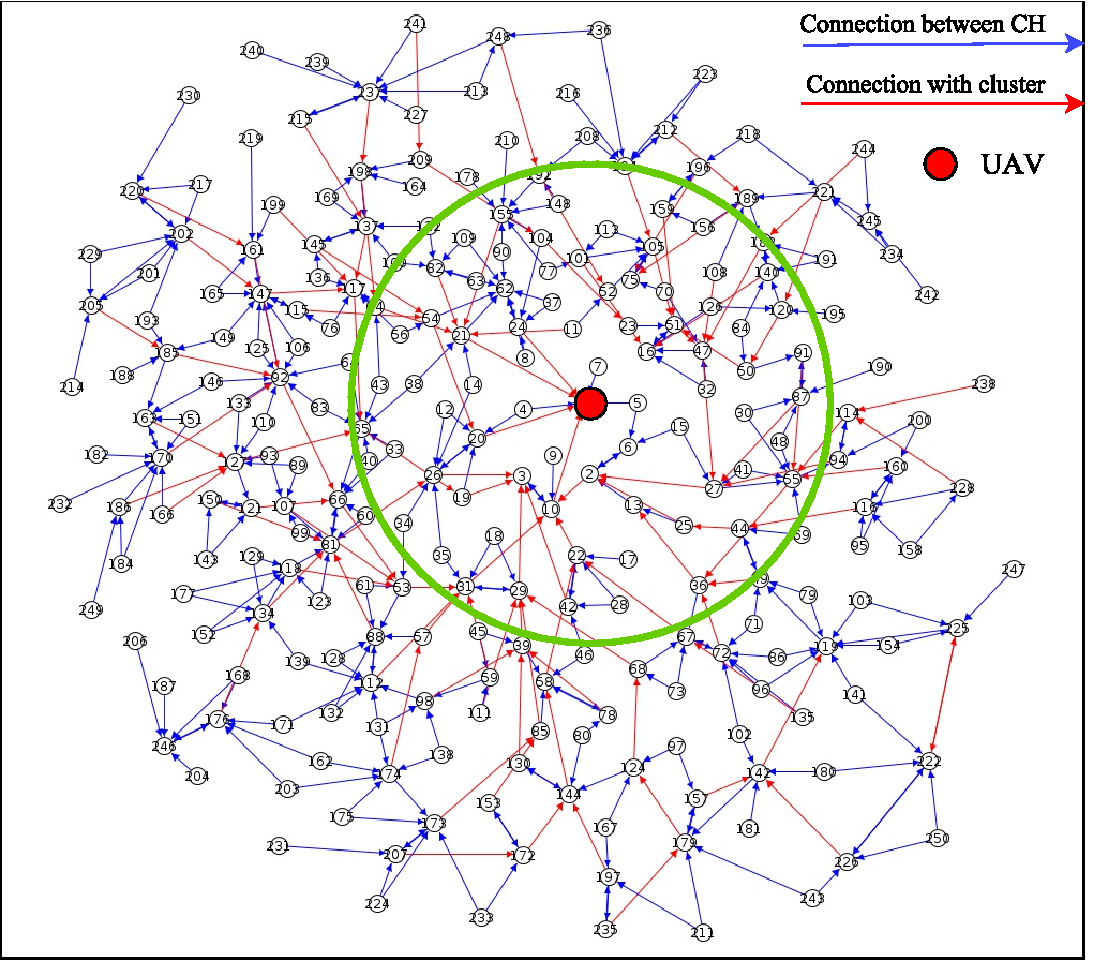
\includegraphics[width=.85\columnwidth]{Figure/topology}
	\vspace{-0.1in}
	\caption{Network Run-time Topology Computed by {\sdn}. \textnormal{The blue lines
represent the connection between cluster members with cluster headers, and the
red lines donate the route between cluster headers deployed by UAV.}}
	
	\label{topology}
	\vspace{-0.1in}
\end{figure}

According to our UAV gathered network run-time topology, we draw Figure~\ref{topology}, the network run-time topology computed by {\sdn}.


\section{Evaluation}
\label{Eva}

\subsection{Evaluation Settup}
In this section, we describle our performance evaluation in simulation and
real-scene experiments. We distribute 100 TI SensorTag sensors in an about
$250~\times~250$ square meters area, with contiki-ng as its operating system. We
use different metrics for various applications and compare our works with other
state-of-the-art works.

\subsection{Evaluation Metrics}

\textbf{Packet recieved ratio} is defined as the proportion of the total data
packets recieved by data sink and the the total data packets sent by all nodes,
and it can be formulated as
\begin{equation}
	L = \frac{\sum_{i = 0}^{N}S_i}{R}
\end{equation}
where $L$ reprents the throughput, and $S_i$ and $R$ denotes the number of
packets sent by the $i$-th node and the number of packets recieved by data
center, respectively.

\textbf{Throughput} is defined as the the total data packets recieved by data
sink, and it measures the capability and scalability of a network.

\textbf{Energy Consumption} is estimated by multipling different coefficients on
CPU running time and radio listening and transmitting time and summing them up.
The coefficients are proportional to the working current described in sensor's
DataSheet. Average energy consumption is the energy consumption of a node in
unit time.

\subsection{Performance}

Figure~\ref{fig:packet_loss_ratio_with_size} shows two remarkable advantages of
{\sdn}: (1) The packet recieved ratio exceeds state-of-the-art
algorithms\cite{winter2012rpl, kaur2016wsn} by 20\%; (2) With the incresing of
network size, the {\sdn}'s packet recieved ration is still much higher than
others'. The reasons are that {\sdn} uses global information to achieve optimal
routing and intelligent cluster header selection balances the energy consumption
between nodes.

\begin{figure}[htbp]
	\centering
	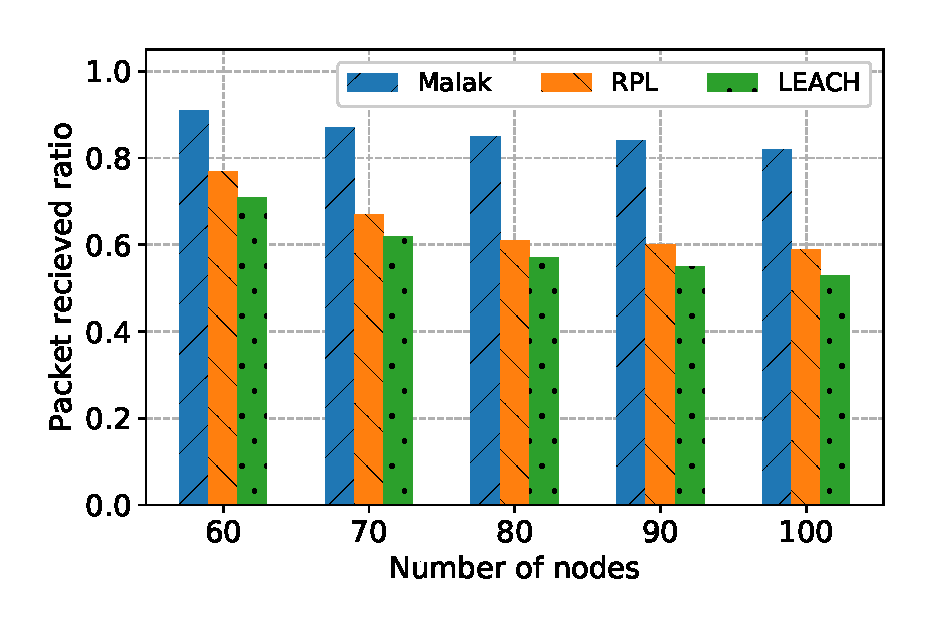
\includegraphics[width=.95\columnwidth]{Figure/packet_loss_ratio_with_size}
	\vspace{-0.1in}
	\caption{Packet recieved ratio
		\textnormal{
		}}
	\label{fig:packet_loss_ratio_with_size}
\end{figure}

Figure~\ref{fig:throughput} compares network throughput by deploying various
routing algorithms. As our {\sdn} uses OSPF, which finds the optimal path from
sensors to data center, to caculate the route table, its throughput exceeds RPL
and LEACH. Besides, in {\sdn}, sensors' lifetime increases a lot more than
others, because all computation-intensive tasks are done by UAV and sensors do
not need to send packets to negotiate route path, which decrease the energy
consumption with no doubt.

\begin{figure}[htbp]
	\centering
	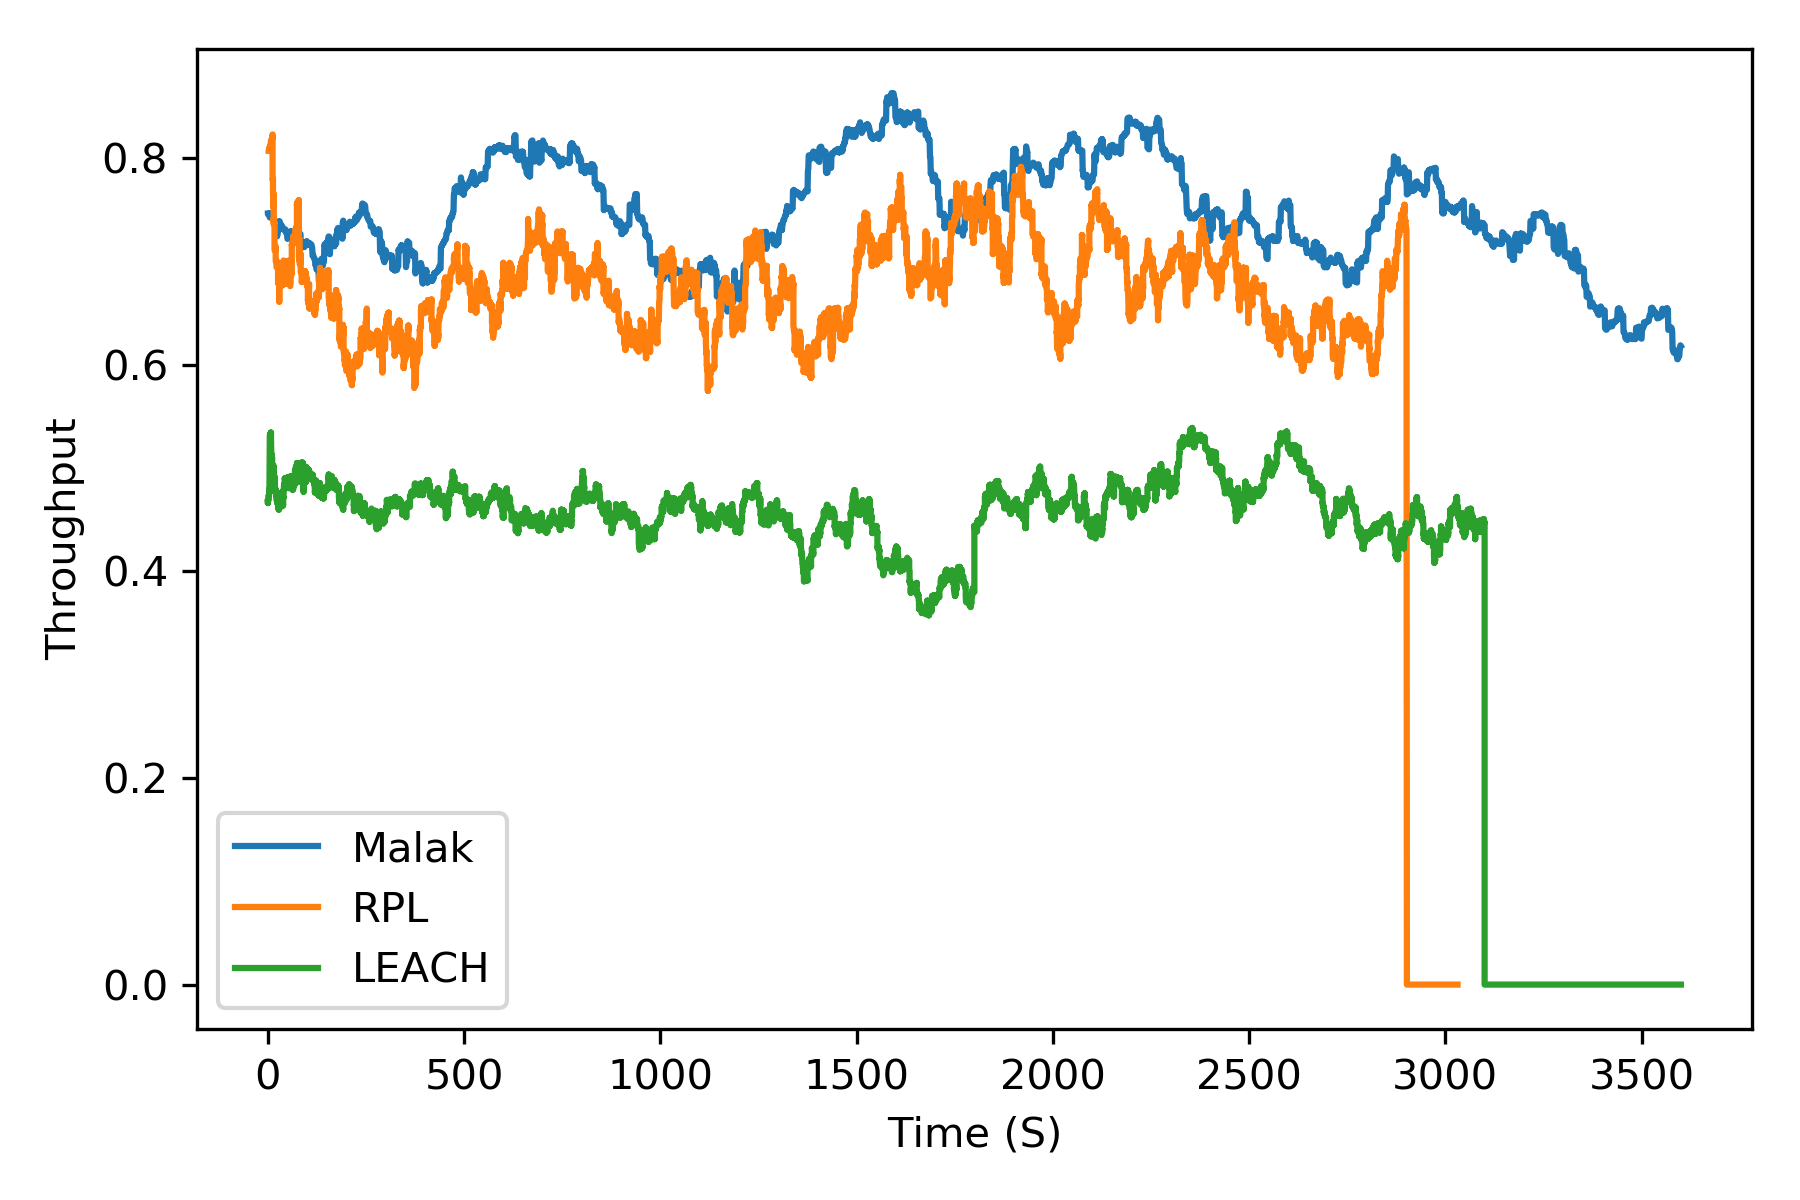
\includegraphics[width=.95\columnwidth]{Figure/throughput}
	\vspace{-0.1in}
	\caption{Routing throughput.
		\textnormal{
			The figure shows throughput corresponding to three kinds of Routing
			algorithms. Throughput can drop to zero when some key nodes are dead
			in the network.
		}}
	\label{fig:throughput}
\end{figure}

\begin{figure}[htbp]
	\centering
	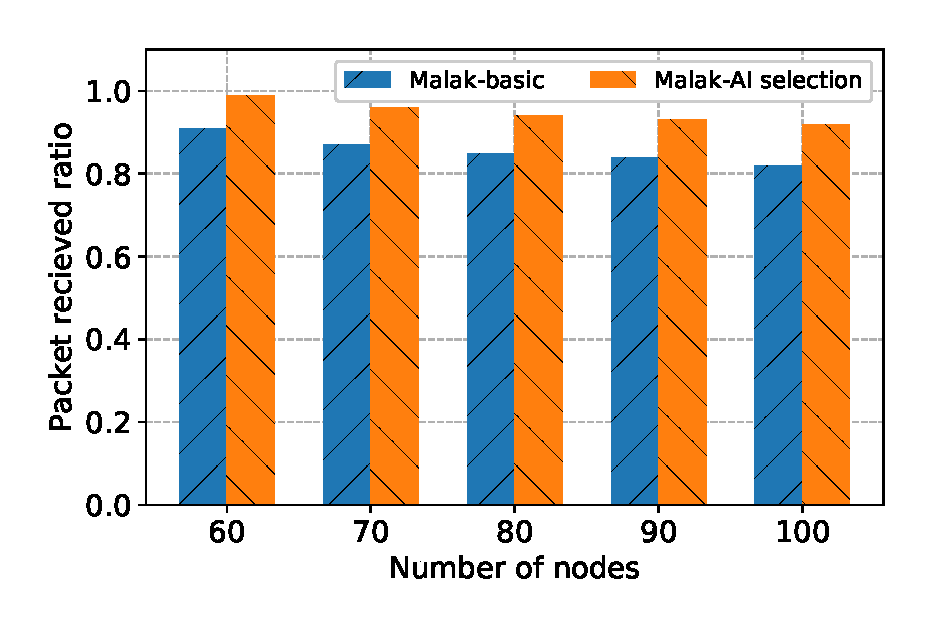
\includegraphics[width=.95\columnwidth]{Figure/ai_selection}
	\vspace{-0.1in}
	\caption{Packet recieved ratio improved by intelligent node selction
		\textnormal{
		}}
	\label{fig:ai_selection}
\end{figure}

\begin{figure}[htbp]
	\centering
	\hspace{-0.3cm}
	\subfloat[Energy prediction]{
		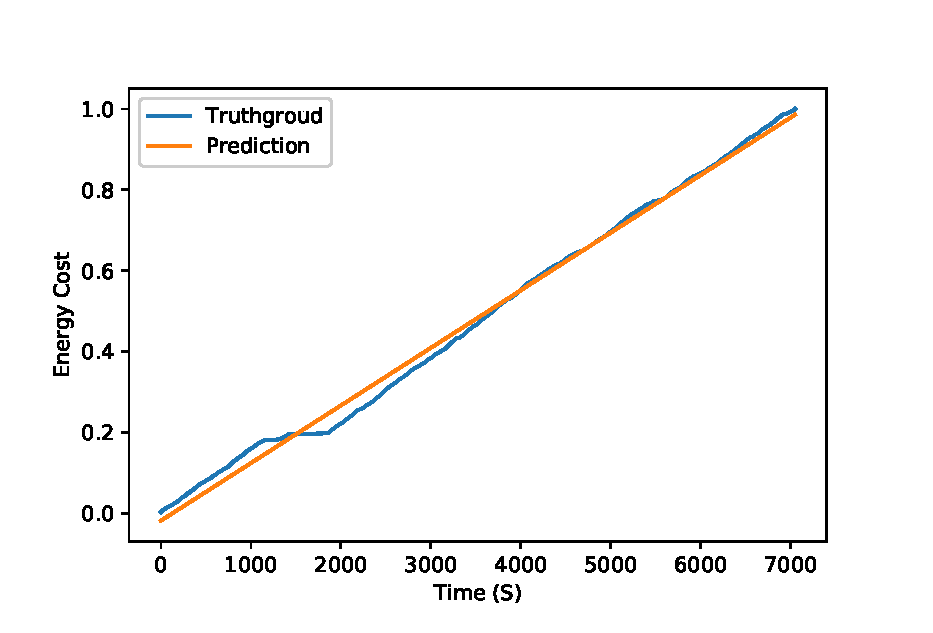
\includegraphics[width=.48\columnwidth]{Figure/energy_pred}
		\label{fig:energy_pred:a}
	}
	\hspace{-0.2cm}
	\subfloat[Prediction error]{
		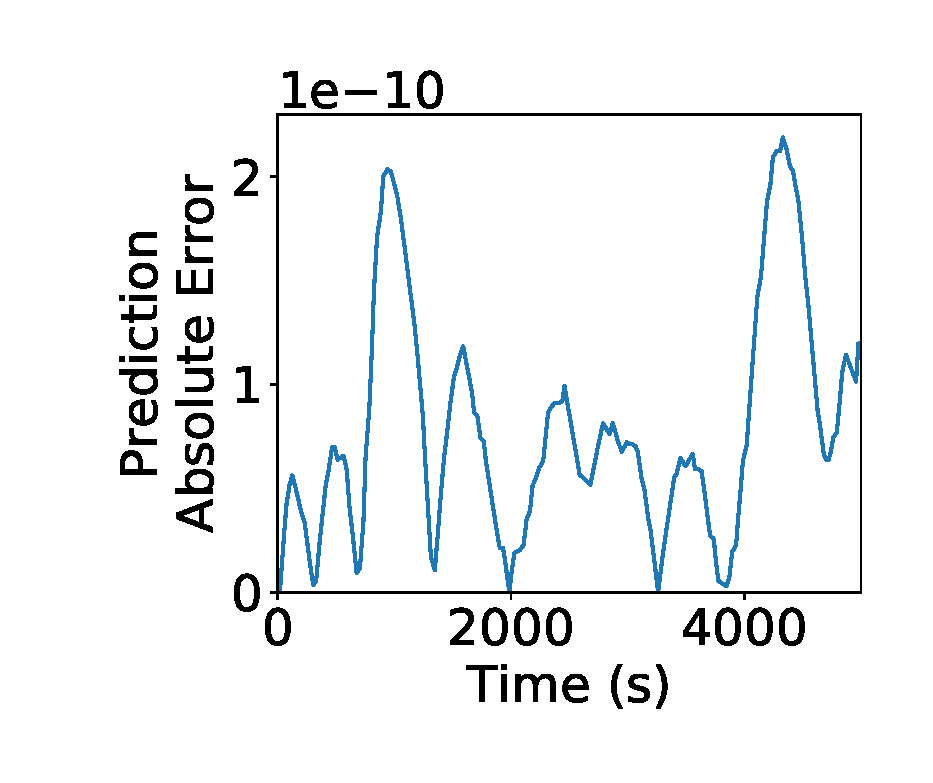
\includegraphics[width=.48\columnwidth]{Figure/energy_pred_err}
		\label{fig:energy_pred:b}
	}
	\vspace{-0.1in}
	\caption{Energy prediction
		\textnormal{
			We use regression method to predict energy consumption and the
			prediction result is consistent with the truthground.  The absolute
			error of energy prediction never exceeds $3\times10^{-10}$ with normalized energy
			(i.e. the maximum energy of a sensor is 1).
		}
	}
	\label{fig:energy_pred}
\end{figure}


\subsection{Resilience}

\begin{figure}[htbp]
	\centering
	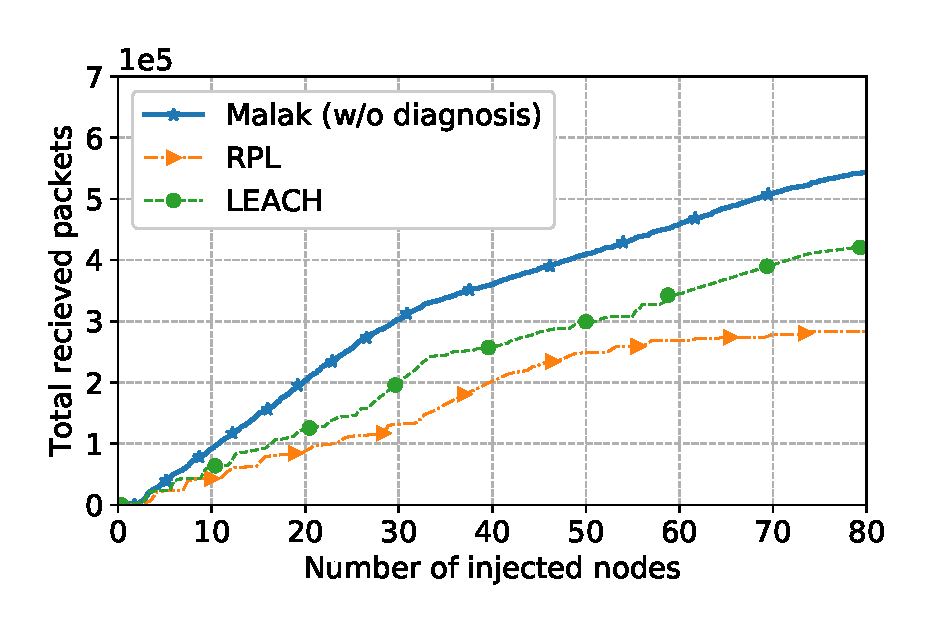
\includegraphics[width=.95\columnwidth]{Figure/fault_tolerance}
	\vspace{-0.1in}
	\caption{Fault tolerance
		\textnormal{
			RPL and {\sdn} are compared on resilience, and {\sdn} perform
			slightly better than RPL.
		}}
	\label{fig:fault_tolerance}
\end{figure}

We compare the impact caused by death of nodes using throughput between RPL and
{\sdn} and the results are shown in Figure~\ref{fig:fault_tolerance}. Throughput
can be low when the number of death is small, because we distribute the sensors
densely and the collision problem is severe. And the throughput grows as some
node died. But after some key nodes died, the throughput falls down quickly,
however, our {\sdn} still performs better than RPL.

\begin{figure}[htbp]
	\centering
	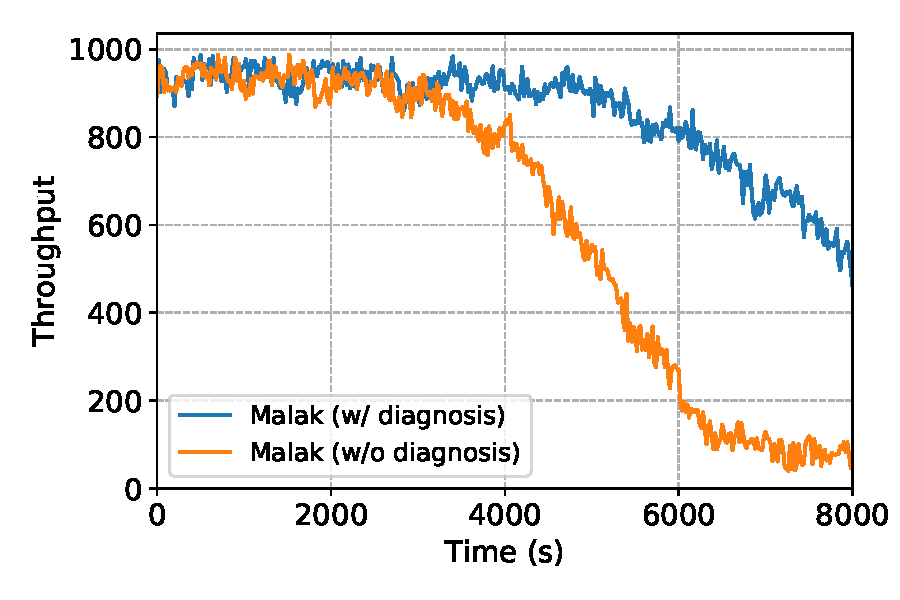
\includegraphics[width=.95\columnwidth]{Figure/diagnosis}
	\vspace{-0.1in}
	\caption{
		\textnormal{
		}}
	\label{fig:diagnosis}
\end{figure}

\begin{table}[htbp]
	\centering
	\caption{Failure detection rate for various failure type and number}
	\label{tab:diagnosis}
	\begin{tabular}{|c||c|c|c|c|c|}
		\hline
		\diagbox{Type}{Failures} & 1 & 2 & 3 & 4 & 5\\
		\hline
		\hline
		Sensing & 98\% & 95\% & 93\% & 92\% & 90\%\\
		\hline
		Energy & 100\% & 93\% & 92\% & 90\% & 88\%\\
		\hline
		Radio & 100\% & 90\% & 88\% & 84\% & 80\%\\
		\hline
	\end{tabular}
\end{table}


\subsection{Energy Consumption}

\begin{figure}[htbp]
	\centering
	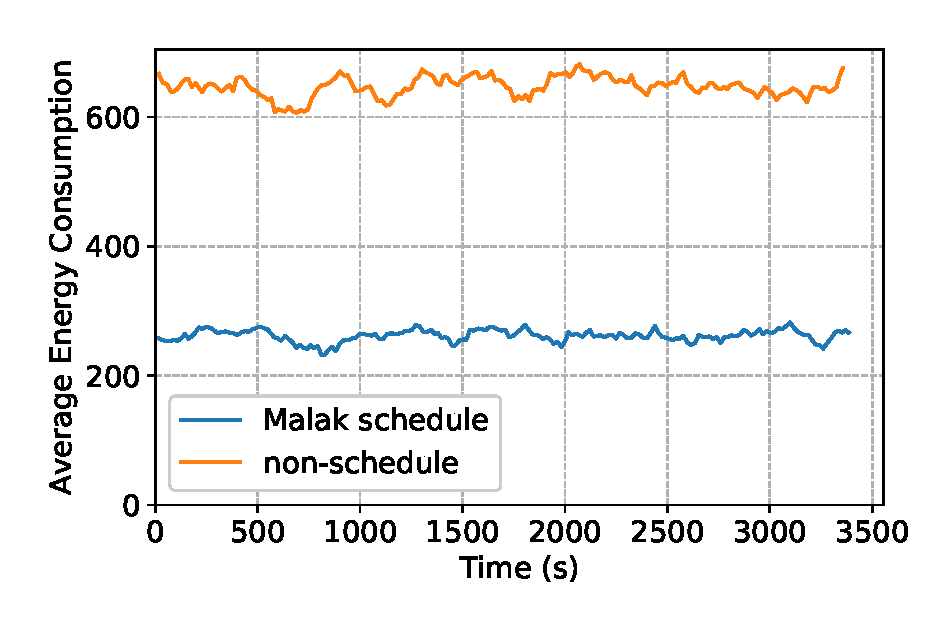
\includegraphics[width=.95\columnwidth]{Figure/multitask_energy}
	\vspace{-0.1in}
	\caption{Average energy consumption with and without multitask schedule
		\textnormal{When with multitask schedule, sensor consumes half of the energy
			comparing to when without multitask schedule.}}
	\label{fig:multitask_energy}
\end{figure}

\subsection{Scalability}

\begin{figure}[htbp]
	\centering
	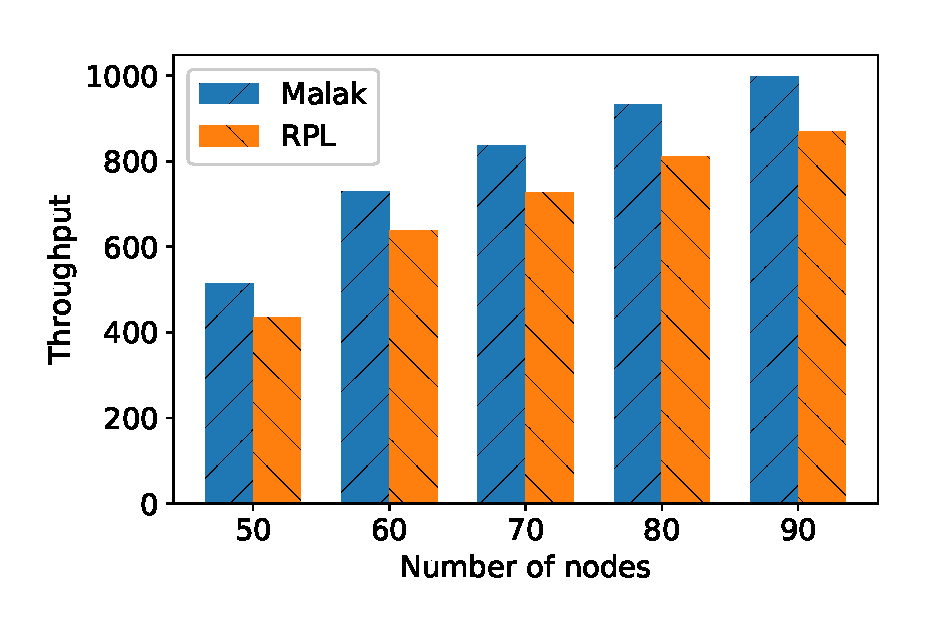
\includegraphics[width=.95\columnwidth]{Figure/scalability}
	\vspace{-0.1in}
	\caption{Scalability
		\textnormal{
			{\sdn} succeeds RPL in different network sizes.
		}}
	\label{fig:scalability}
\end{figure}


\section{Conclusion}
\label{Con}

Conclusion goes here.


\bibliographystyle{acm}
\bibliography{Ref}

\end{document}
